To adjust the brightness of your image, you can scale all of the intensity values by a multiplicative factor down (towards darker values) or up (towards brighter values). Based on looking at the histogram, should your image be brightened? Dimmed? Why?

\begin{solution}
    The original image looks fairly well distributed, but is slightly skewed to the left. This can be adjusted by slightly increasing the intensity.
    
    \begin{lstlisting}[language=Matlab]
    X_gray_adj = X_gray * 1.1;
    imshow(X_gray_adj)
    \end{lstlisting}
    
    \begin{center}
        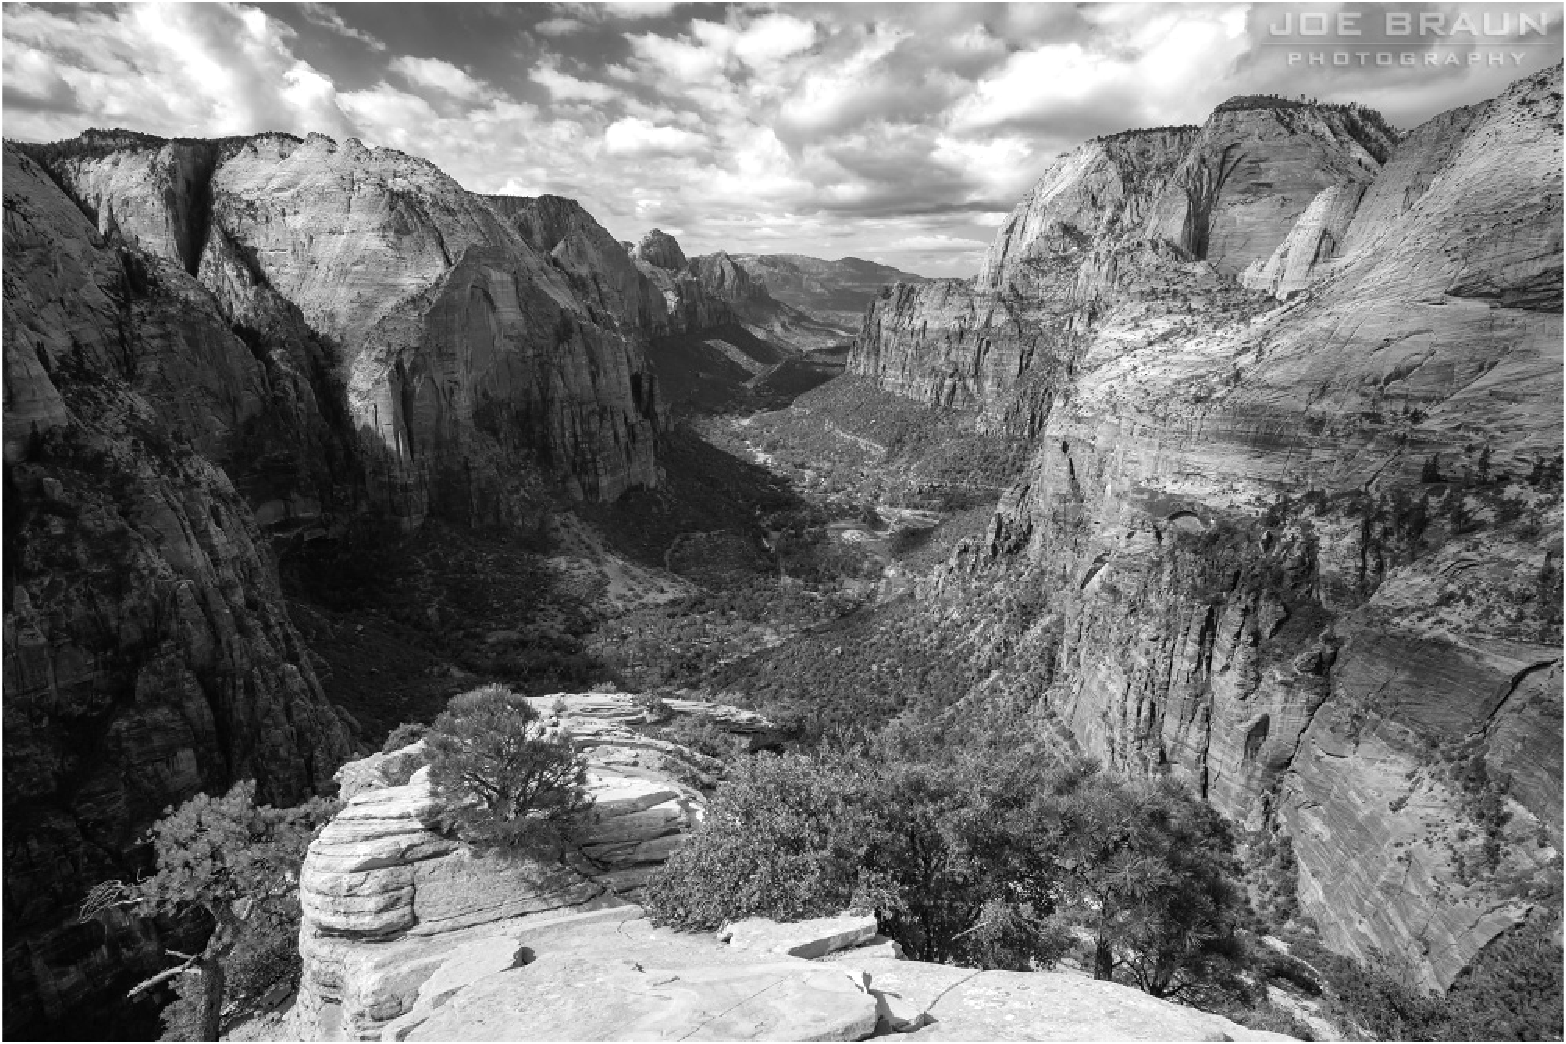
\includegraphics[width=0.5\textwidth]{img/e7p6_img.png}
    \end{center}
    
    \begin{lstlisting}[language=Matlab]
    histogram(X_gray_adj)
    \end{lstlisting}
    
    \begin{center}
        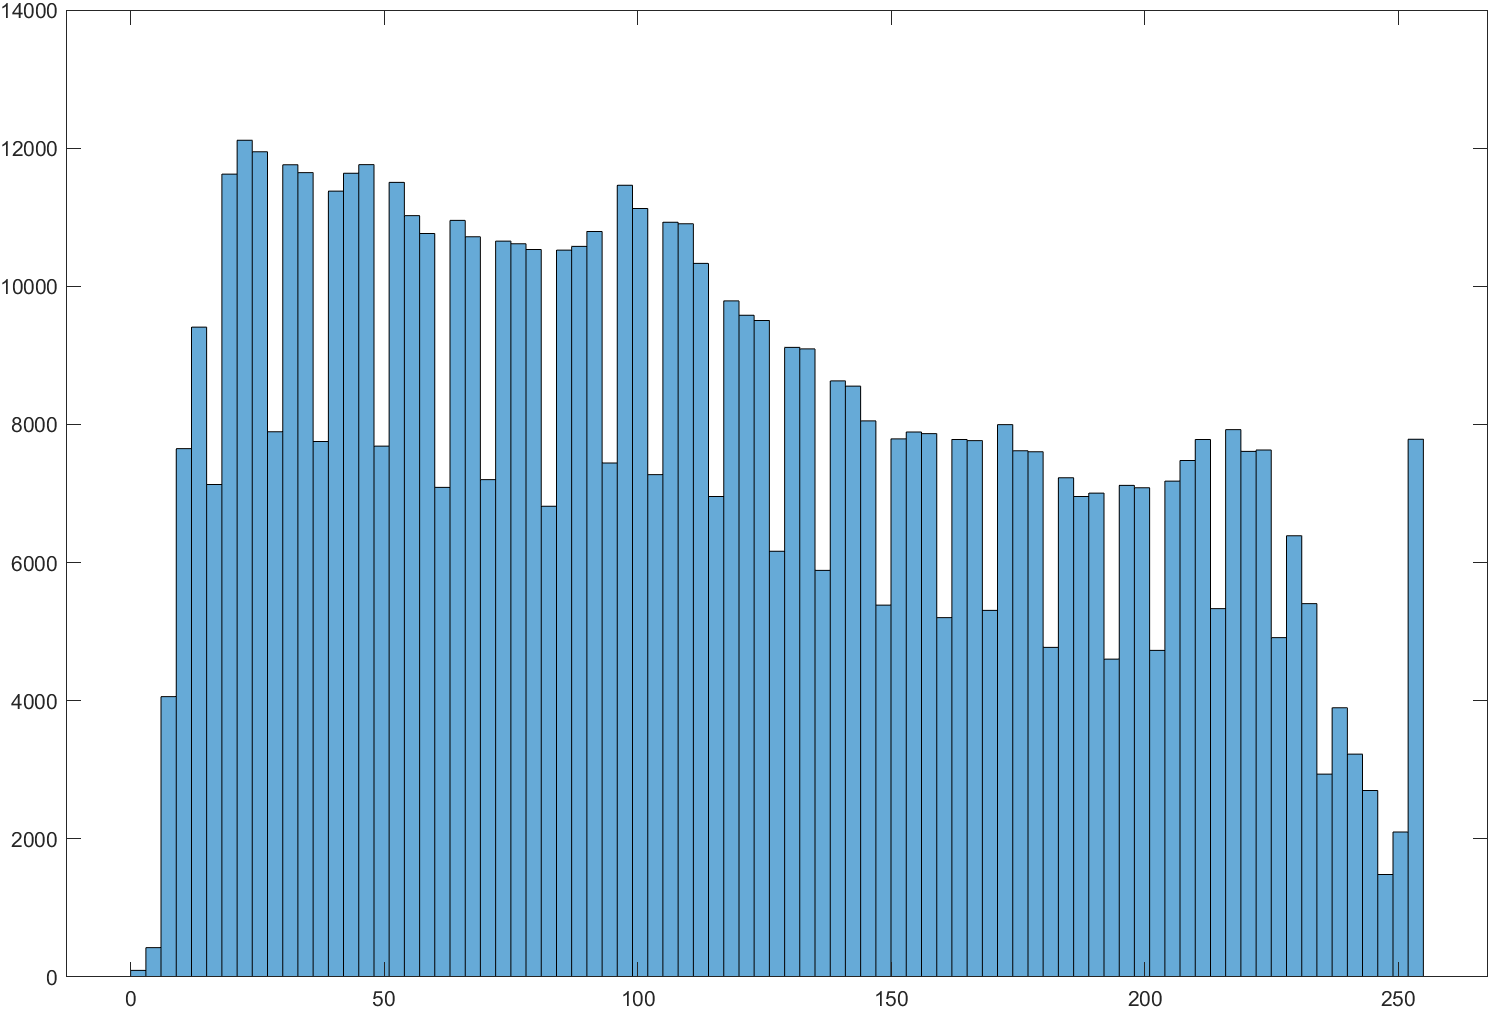
\includegraphics[width=0.8\textwidth]{img/e7p6_hist.png}
    \end{center}
    
    The intensity histogram looks a lot more well distributed with a factor of 1.1, but it also indicates a significant amount of saturation. My guess of where that saturation is in the clouds.
\end{solution}